\subsection{Sprint 2}

\subsubsection{Logical Lines Of Code (LLOC)}
\label{section:sprint2LLOC}

\begin{figure}
\centering
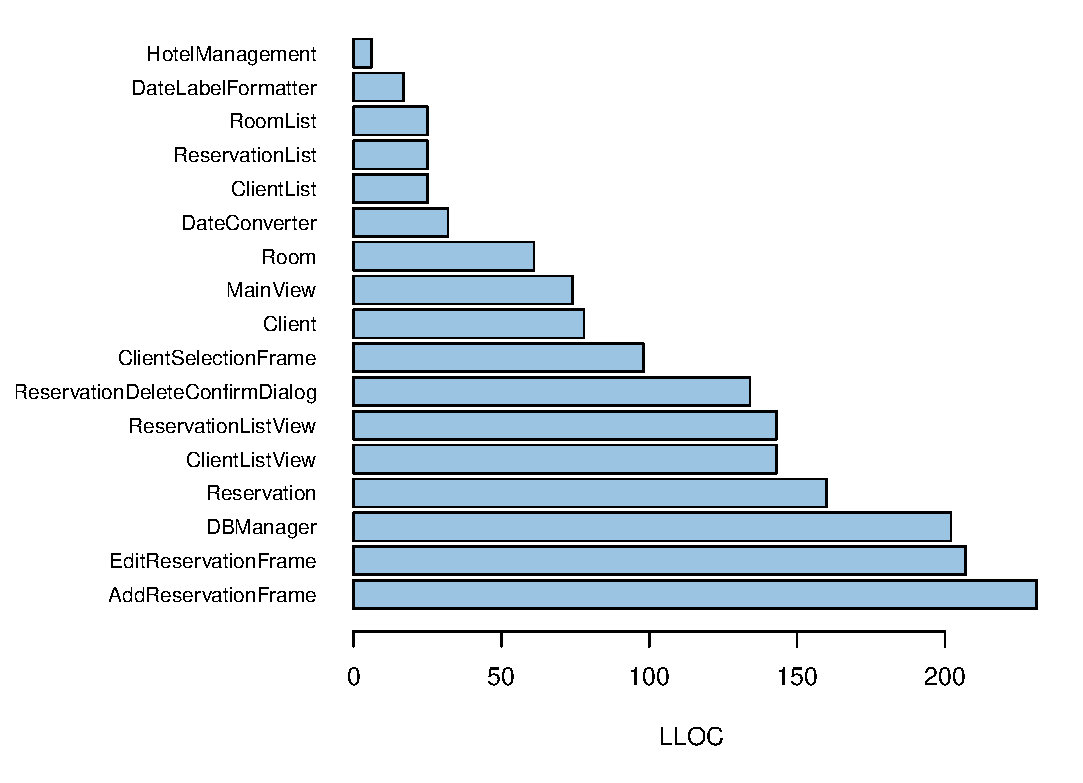
\includegraphics[width=1.0\textwidth]{Sprint2-LLOC-1.eps}
\caption{Λογικές γραμμές κώδικα ανά κλάση στο τέλος του sprint 2}
\label{fig:sprint2LLOC}
\end{figure}

\subsubsection{Clone Coverage (CC)}
\label{section:sprint2CC}

\begin{figure}
\centering
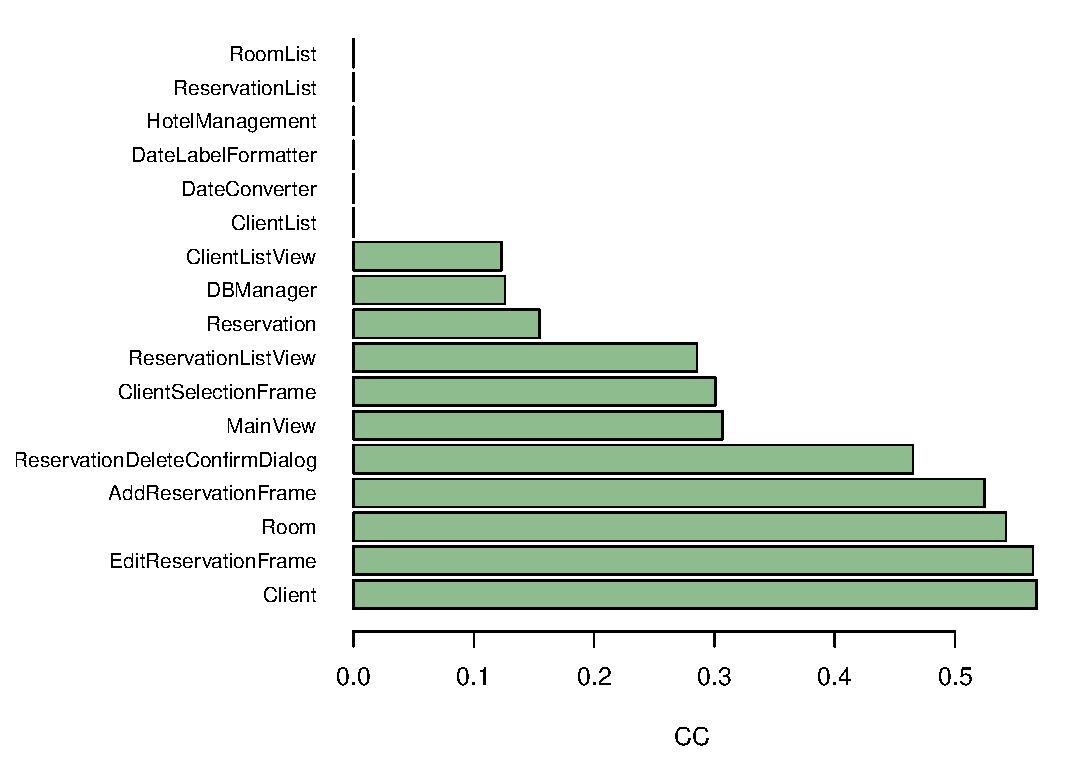
\includegraphics[width=1.0\textwidth]{Sprint2-CC-1.eps}
\caption{Τιμές της μετρικής CC ανά κλάση στο τέλος του sprint 2}
\label{fig:sprint2CC}
\end{figure}

\subsubsection{McCabe’s Cyclomatic Complexity (McCC)}
\label{section:sprint2McCC}

\begin{figure}
\centering
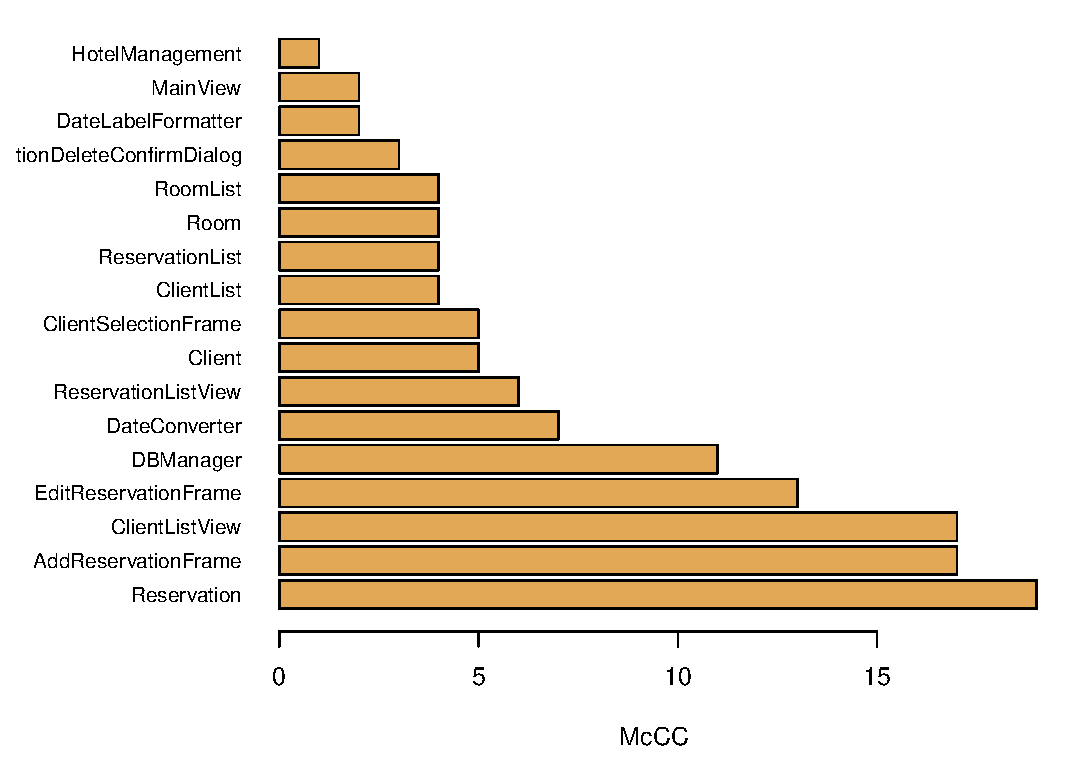
\includegraphics[width=1.0\textwidth]{Sprint2-McCC-1.eps}
\caption{Τιμές της μετρικής κυκλωματικής πολυπλοκότητας McCC ανά κλάση στο τέλος του sprint 2}
\label{fig:sprint2McCC}
\end{figure}

\subsubsection{Lack of Cohesion in Methods 5 (LCOM5)}
\label{section:sprint2LCOM5}

\begin{figure}
\centering
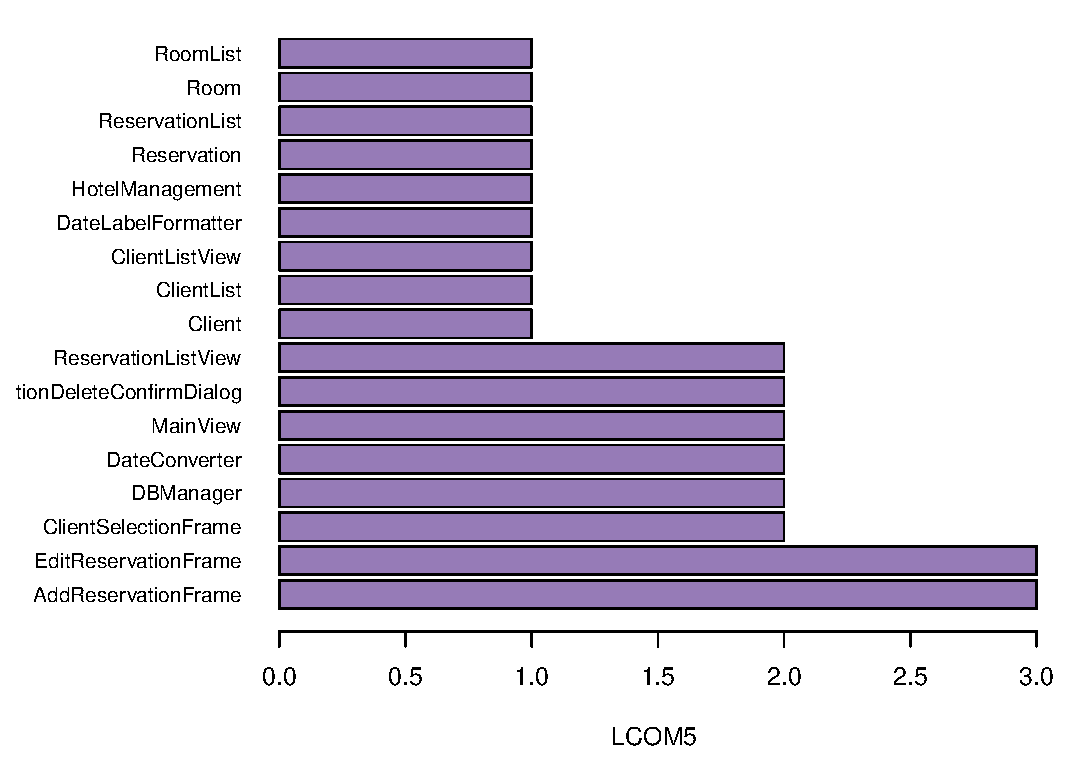
\includegraphics[width=1.0\textwidth]{Sprint2-LCOM5-1.eps}
\caption{Τιμές της μετρικής έλλειψης συνεκτικότητας LCOM5 ανά κλάση στο τέλος του sprint 2}
\label{fig:sprint2LCOM5}
\end{figure}

\subsubsection{Coupling Between Object classes (CBO)}
\label{section:sprint2CBO}

\begin{figure}
\centering
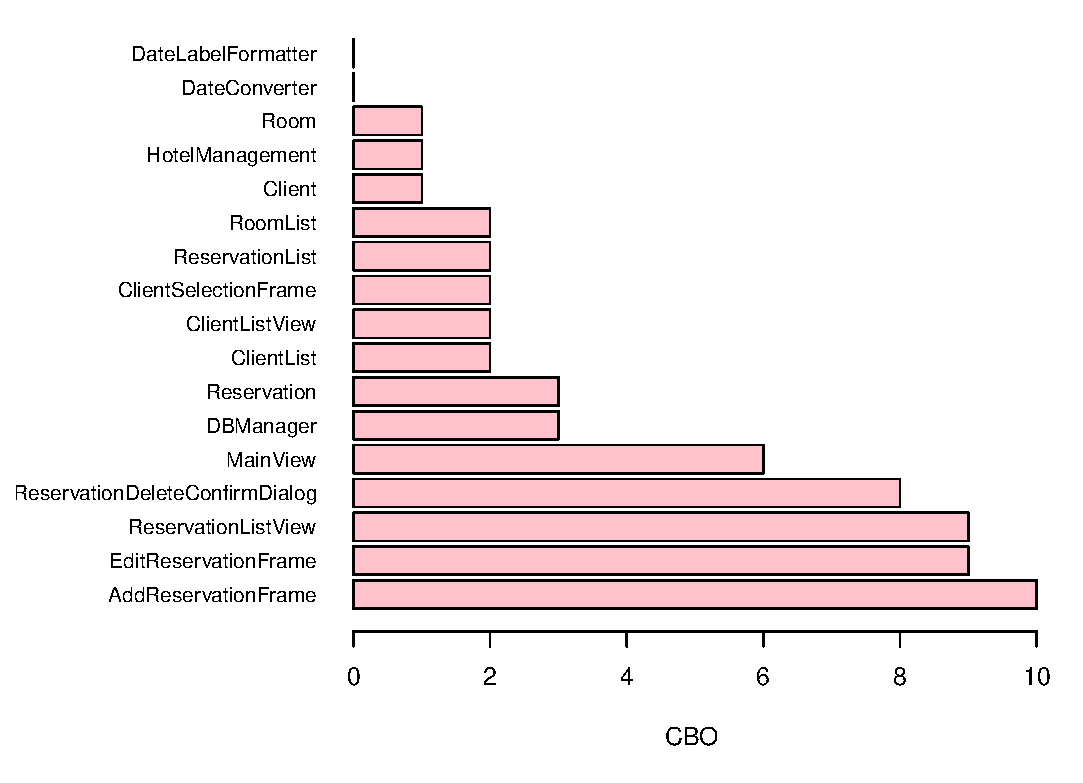
\includegraphics[width=1.0\textwidth]{Sprint2-CBO-1.eps}
\caption{Τιμές της μετρικής σύζευξης CBO ανά κλάση στο τέλος του sprint 2}
\label{fig:sprint2CBO}
\end{figure}
